\documentclass[conference]{IEEEtran}
\IEEEoverridecommandlockouts
% The preceding line is only needed to identify funding in the first footnote. If that is unneeded, please comment it out.
%Template version as of 6/27/2024

\usepackage{cite}
\usepackage{amsmath,amssymb,amsfonts}
\usepackage{pxfonts}
\usepackage{algorithmic}
\usepackage{graphicx}
\usepackage{textcomp}
\usepackage{listings}
\usepackage{multicol}
\usepackage{xcolor}
\usepackage[main=brazil,english]{babel}
\def\BibTeX{{\rm B\kern-.05em{\sc i\kern-.025em b}\kern-.08em
    T\kern-.1667em\lower.7ex\hbox{E}\kern-.125emX}}

% Código fonte MATLAB
\definecolor{darkgreen}{rgb}{0.0, 0.5, 0.0}
\renewcommand{\lstlistingname}{Código}
\lstset{
	basicstyle=\ttfamily\footnotesize, % Fonte monoespaçada e pequena
	numbers=none,                     % Números de linha à esquerda
	numberstyle=\tiny,                % Tamanho dos números de linha
	stepnumber=1,                     % Incremento dos números
	numbersep=5pt,                    % Distância dos números para o código
	backgroundcolor=\color{lightgray!10}, % Fundo cinza claro
	frame=single,                     % Moldura ao redor do código
	tabsize=4,                        % Tamanho da tabulação
	captionpos=b,                     % Posição da legenda (bottom)
	breaklines=true,                  % Quebra de linha automática
	breakatwhitespace=false,          % Quebra de linha mesmo no meio de palavras
	showspaces=false,                 % Não mostrar espaços
	showstringspaces=false,           % Não mostrar espaços em strings
	keywordstyle=\color{blue},        % Cor para palavras-chave
	commentstyle=\color{darkgreen},       % Cor para comentários
	stringstyle=\color{purple},       % Cor para strings
	language=Matlab                   % Linguagem do código
}

\begin{document}

\title{
	%Aplicação de CNNs no reconhecimento de gestos a partir de sinais de sEMG
	%Revisão da aplicação de CNN no reconhecimento de sinais de sEMG
	%Reconhecimento de gestos a partir de sinais sEMG: uma revisão de aplicações de CNN
	%Uso de CNNs para reconhecimento de gestos a partir de sinais sEMG
	%Uso de CNNs para reconhecimento de gestos a partir de sinais sEMG: revisão
	%Revisão da arquitetura CNN para aplicações de sEMG: resultados e observações
	%2.
	%Reconhecimento de gestos por sEMG: uma análise da eficiência de arquiteturas de CNNs
	%Avanço no reconhecimento de gestos por sEMG: uma revisão de desempenho de CNNs
	%1.
	%Eficiência de CNNs no reconhecimento de gestos por sEMG: uma revisão de estudos recentes
	%3.
	%CNNs aplicadas ao reconhecimento de gestos por sEMG: Avaliação de desempenho e eficiência
	%4.
	%Reconhecimento de gestos por sEMG: uma análise da eficiência de CNNs em estudos recentes
	%5
	%Reconhecimento de gestos por sEMG com CNNs: uma análise de eficiência em estudos recentes
	%6
	%Reconhecimento de Gestos por sEMG: Uma Análise da Eficiência de CNNs 
	%7
	Processamento de Imagens para Detecção de Furos em Bicos Injetores Diesel
	%Panorama da eficiência em reconhecimento de gestos por sEMG: uma revisão de abordagens com CNNs
	 
%{\footnotesize \textsuperscript{*}Note: Sub-titles are not captured for https://ieeexplore.ieee.org  and
%should not be used}
%\thanks{Identify applicable funding agency here. If none, delete this.}
}

\author{
	\IEEEauthorblockN{
		1\textsuperscript{st}
		Wellinthon da Silveira Kiiller
	}
	\IEEEauthorblockA{
		\textit{Programa de Pós-Graduação em Engenharia Elétrica e
		Informática Industrial (CPGEI-CT)} \\
		\textit{Universidade Tecnológica Federal do Paraná (UTFPR)}\\
		Curitiba, Paraná, Brasil \\
		https://orcid.org/0009-0000-8591-0393
	}
	%\and
	%\IEEEauthorblockN{2\textsuperscript{nd} Given Name Surname}
	%\IEEEauthorblockA{\textit{dept. name of organization (of Aff.)} \\
	%\textit{name of organization (of Aff.)}\\
	%City, Country \\
	%email address or ORCID}
}

\maketitle

% Linguagem: português
%\selectlanguage{brazil}
%\renewcommand\IEEEkeywordsname{Palavras-chave}
%\begin{abstract}
	%Contexto e motivação
	%O que é o tema e por que ele é importante?
	%O reconhecimento de gestos a partir de sinais de eletromiografia de superfície (sEMG) tem ganhado destaque em aplicações biomédicas, especialmente no controle de próteses e em sistemas de reabilitação.	
	%Objetivo do trabalho
	%O que você fez? Qual era o propósito principal?
	%Esse trabalho investiga a aplicação de redes neurais convolucionais (CNNs) na identificação e classificação de gestos com base em sinais de sEMG.	
	%Metodologia usada
	%Como você fez? Qual foi a abordagem geral?
	%Por meio de uma revisão de literatura, são analisadas arquiteturas de CNN comumente empregadas na área, como ResNet-50, VGGNet-11 e GoogLeNet, considerando diferentes métodos de pré-processamento e representação dos sinais em imagens. Além disso, são discutidas técnicas como \textit{sliding window} e transformadas tempo-frequência, incluindo a \textit{Short-Time Fourier Transform} (STFT).
	%Principais resultados (se houver)
	%Quais foram os achados mais relevantes?
	%(Se não houver resultados ainda, diga o que o artigo apresenta.)
	%Os resultados apresentados em pesquisas recentes fortalecem o alto potencial das CNNs em alcançar acurácias superiores a 90\% no reconhecimento de padrões gestuais, com perspectivas promissoras para aplicações em tempo real.
	%Conclusão ou contribuição
	%O que esse trabalho oferece à área? Qual é a contribuição?
	%Por fim, esse trabalho oferece uma base metodológica sólida, servindo como referência para futuras implementações de sistemas de reconhecimento de movimentos baseados em sEMG.
%\end{abstract}

%\begin{IEEEkeywords}
%CNN, sEMG, classificação de gestos, reconhecimento de padrões.
%\end{IEEEkeywords}

% Linguagem: português
\selectlanguage{brazil}

\section{Introducão}

Os bicos injetores desempenham uma função fundamental nos sistemas de combustão a diesel. Em uma multinacional especializada na produção desses bicos, é essencial assegurar a rastreabilidade do produto ao longo dos diversos processos de fabricação. Uma forma eficaz de garantir a rastreabilidade é por meio de gravações a laser, que, ao contrário de etiquetas ou adesivos, permanece intacta durante o processo de fabricação.

Nesse contexto, este trabalho tem como objetivo demonstrar a aplicação de técnicas de processamento de imagens para detectar furos na superfície de vedação de bicos injetores diesel, uma área estratégica para a gravação a laser com fins de rastreabilidade. O artigo está organizado da seguinte forma: na Seção 2.A, é apresentada uma breve explicação sobre os bicos injetores; an Seção 2.B, são descritas as técnicas de processamento de imagens utilizadas; por fim, a Seção de Considerações Finais encerra o artigo, destacando as contribuições do estudo.

\section{Materiais e Métodos}
\subsection{Bico Injetor Diesel}

A Figura \ref{fig:bico-injetor-real} ilustra um modelo de bico injetor, um dos principais componentes de um sistema de combustão a diesel. Como o foco deste trabalho é a aplicação de técnicas de processamento de imagens, o funcionamento do bico injetor não será abordado em detalhes. No entanto, a Figura \ref{fig:bico-injetor} destaca alguns de seus componentes.

\begin{figure}[b]
	\centering
	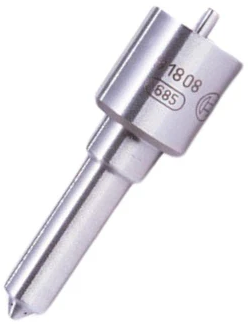
\includegraphics[scale=0.46]{Images/bico-injetor-real.png}
	\caption{Bico injetor diesel. Fonte: \cite{karhub}.}
	\label{fig:bico-injetor-real}
\end{figure}

A Figura \ref{fig:bico-injetor} destaca as seguintes regiões do bico injetor: base (1), haste (2), cúpula (3), furos de fixação (4 e 5), furo de injeção de combustível (6), guia do corpo (7), furo cego (8), assento da agulha (9), ponta da agulha (10), guia da agulha (11) e espiga da agulha (12) \cite{Girotto2023}. Os furos de fixação (4 e 5) e injeção de combustível (6) estão localizados em uma região chamada de superfície de vedação, conforme ilustra a Figura \ref{fig:superficie-de-vedacao}.
 
\begin{figure}[t]
	\centering
	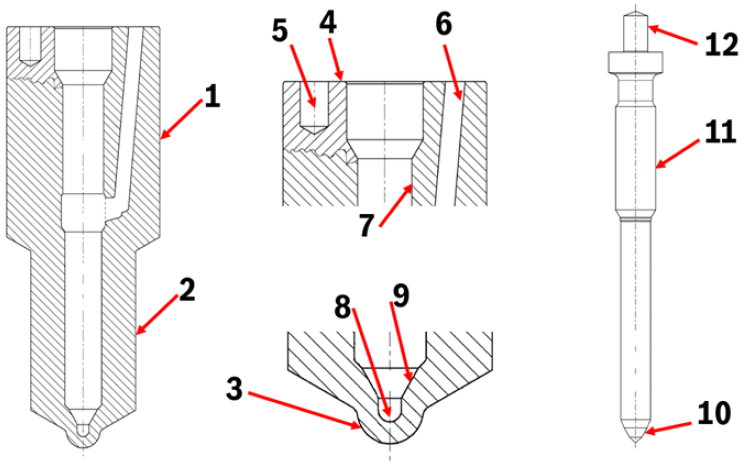
\includegraphics[scale=0.35]{Images/bico-injetor.png}
	\caption{Componentes de um bico injetor diesel. Fonte: \cite{Girotto2023}.}
	\label{fig:bico-injetor}
\end{figure}

\begin{figure}[t]
	\centering
	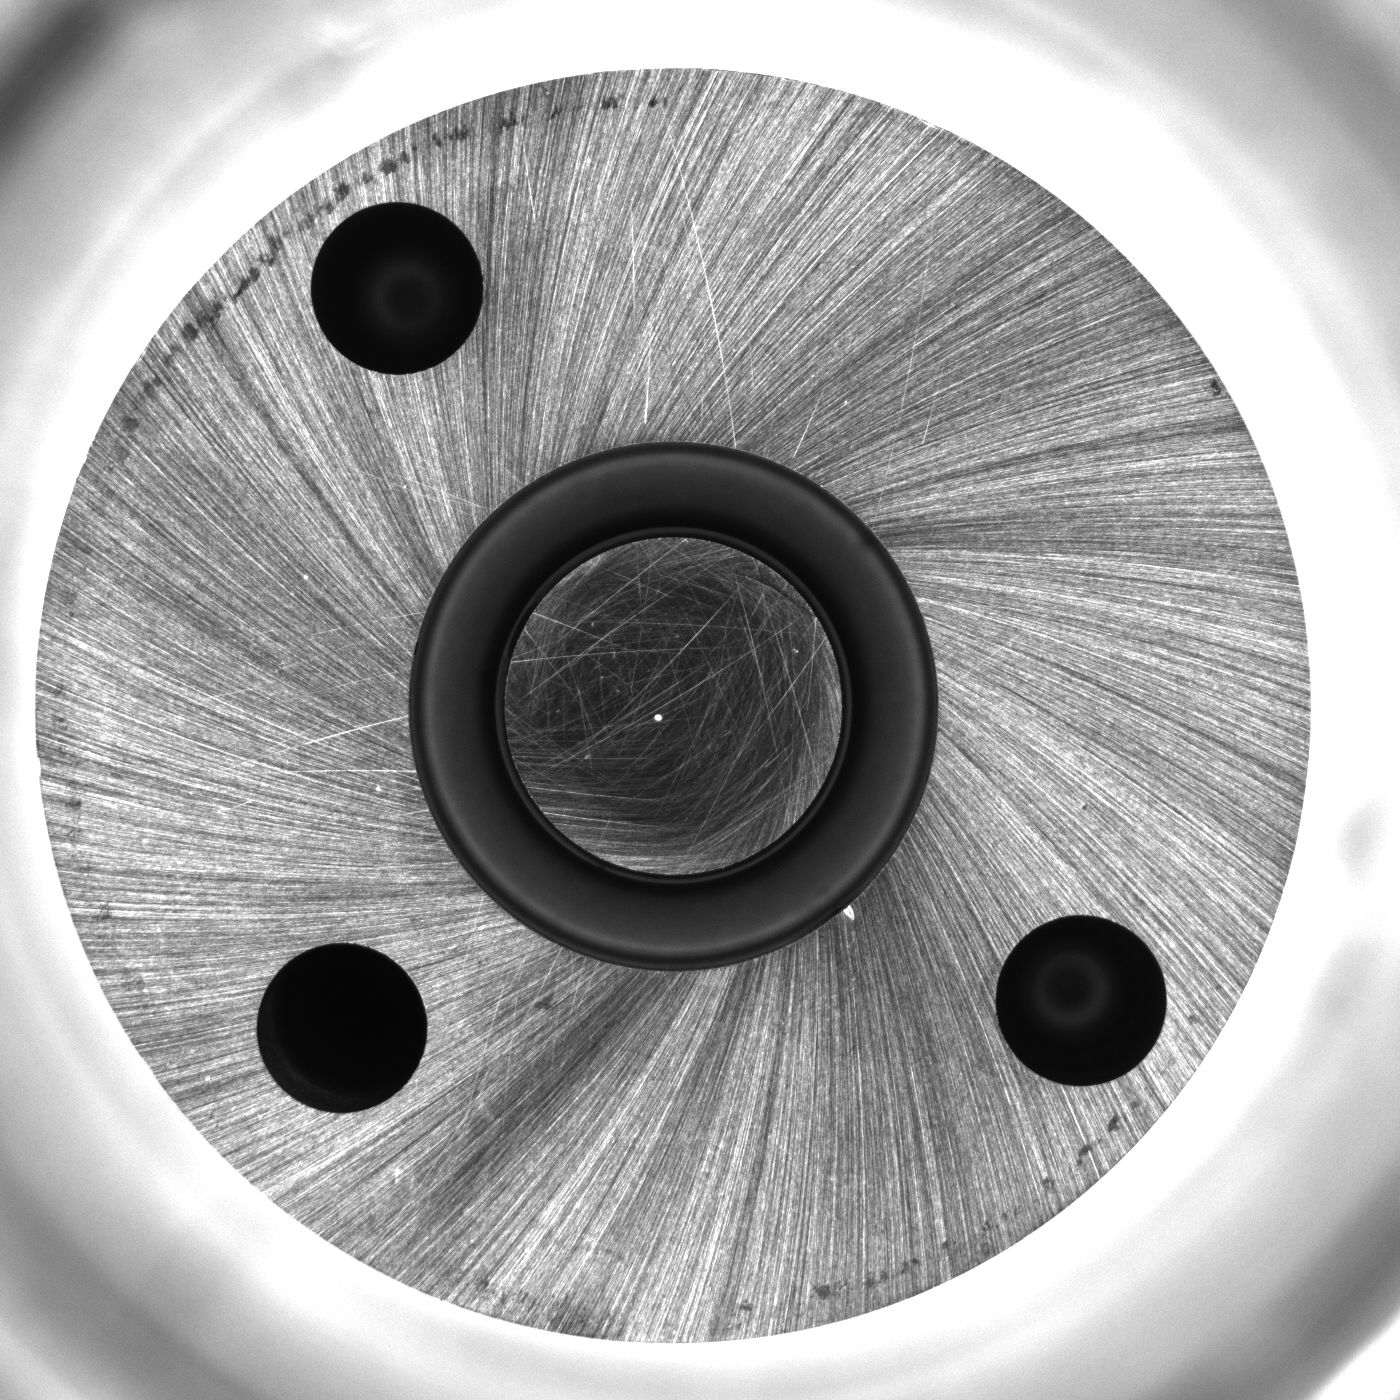
\includegraphics[scale=0.11]{Images/superficie-de-vedacao.jpg}
	\caption{Superfície de vedação de um bico injetor diesel}
	\label{fig:superficie-de-vedacao}
\end{figure}

\subsection{Materiais}

Para a aplicação das técnicas de processamento de imagens, foram desenvolvidos \textit{scripts} em Matlab, executados em um computador pessoal com as seguintes especificações: processador Intel Core i7-7500U de 2 núcleos a 2,90GHz; 16GB de memória RAM; placa de vídeo NVIDIA GeForce 940MX com 4GB de memória dedicada; e sistema operacional Windows 10 Home. 

\subsection{Processamento de Imagens}

Nesta seção, são detalhadas as técnicas de processamento de imagem utilizadas para detecção dos furos presentes na superfície de vedação do bico injetor, utilizando o \textit{software} Matlab.  

\subsubsection{Carregar imagem} esta seção de código descreve as etapas para o carregamento e a visualização da imagem. No Código \ref{lst:codigo-read-image} apresentado, foi carregada uma imagem correspondente à Figura \ref{fig:superficie-de-vedacao}. 

\begin{lstlisting}[caption={Carregamento e visualização da imagem}, label={lst:codigo-read-image}]
% Clear workspace
clear

% Set working directory
workDir = pwd + "/ProjetoFinal/Images/";

% Read image
imName = "Image0001.jpg";
imNozzle = imread(workDir + imName);

% Show image
figure; imshow(imNozzle);
title(imName);
\end{lstlisting}

\subsubsection{Filtrar a imagem} esta seção de código apresenta as etapas de pré-processamento da imagem, utilizando filtros, conforme demonstrado no Código \ref{lst:codigo-filtering}. Inicialmente, foi construído um elemento estrutural em formato de disco por meio da função \textit{strel} para aplicação do filtro. Em seguida, o elemento foi utilizado em um filtro de \textit{closing}, gerando a imagem apresentada na Figura \ref{fig:imClosed}. Por fim, foi implementado um laço \textit{for} para determinar o valor de sensibilidade mais adequado para a binarização da imagem, utilizando a função \textit{imbinarize}. A Figura \ref{fig:sensivities} apresenta as imagens binarizadas obtidas com diferentes valores de sensibilidade.

\begin{lstlisting}[caption={Filtragem e análise da sensibilidade para binarização}, label={lst:codigo-filtering}]
% Create structuring element
se = strel('disk', 3);

% Apply closing morphology and show image
imClosed = imclose(imNozzle, se);
figure; imshow(imClosed);
title('Closed');

% Show binarized images with different sensitivities
% Increment sensitivity by 0.1
figure;
for i=0.1:0.1:1.0
	imBinarized = imbinarize(imClosed, ...
	"adaptive", "Sensitivity", i); 
	subplot(2, 5, i*10); imshow(imBinarized);
	title(i);
end
\end{lstlisting}

\begin{figure}[h]
	\centering
	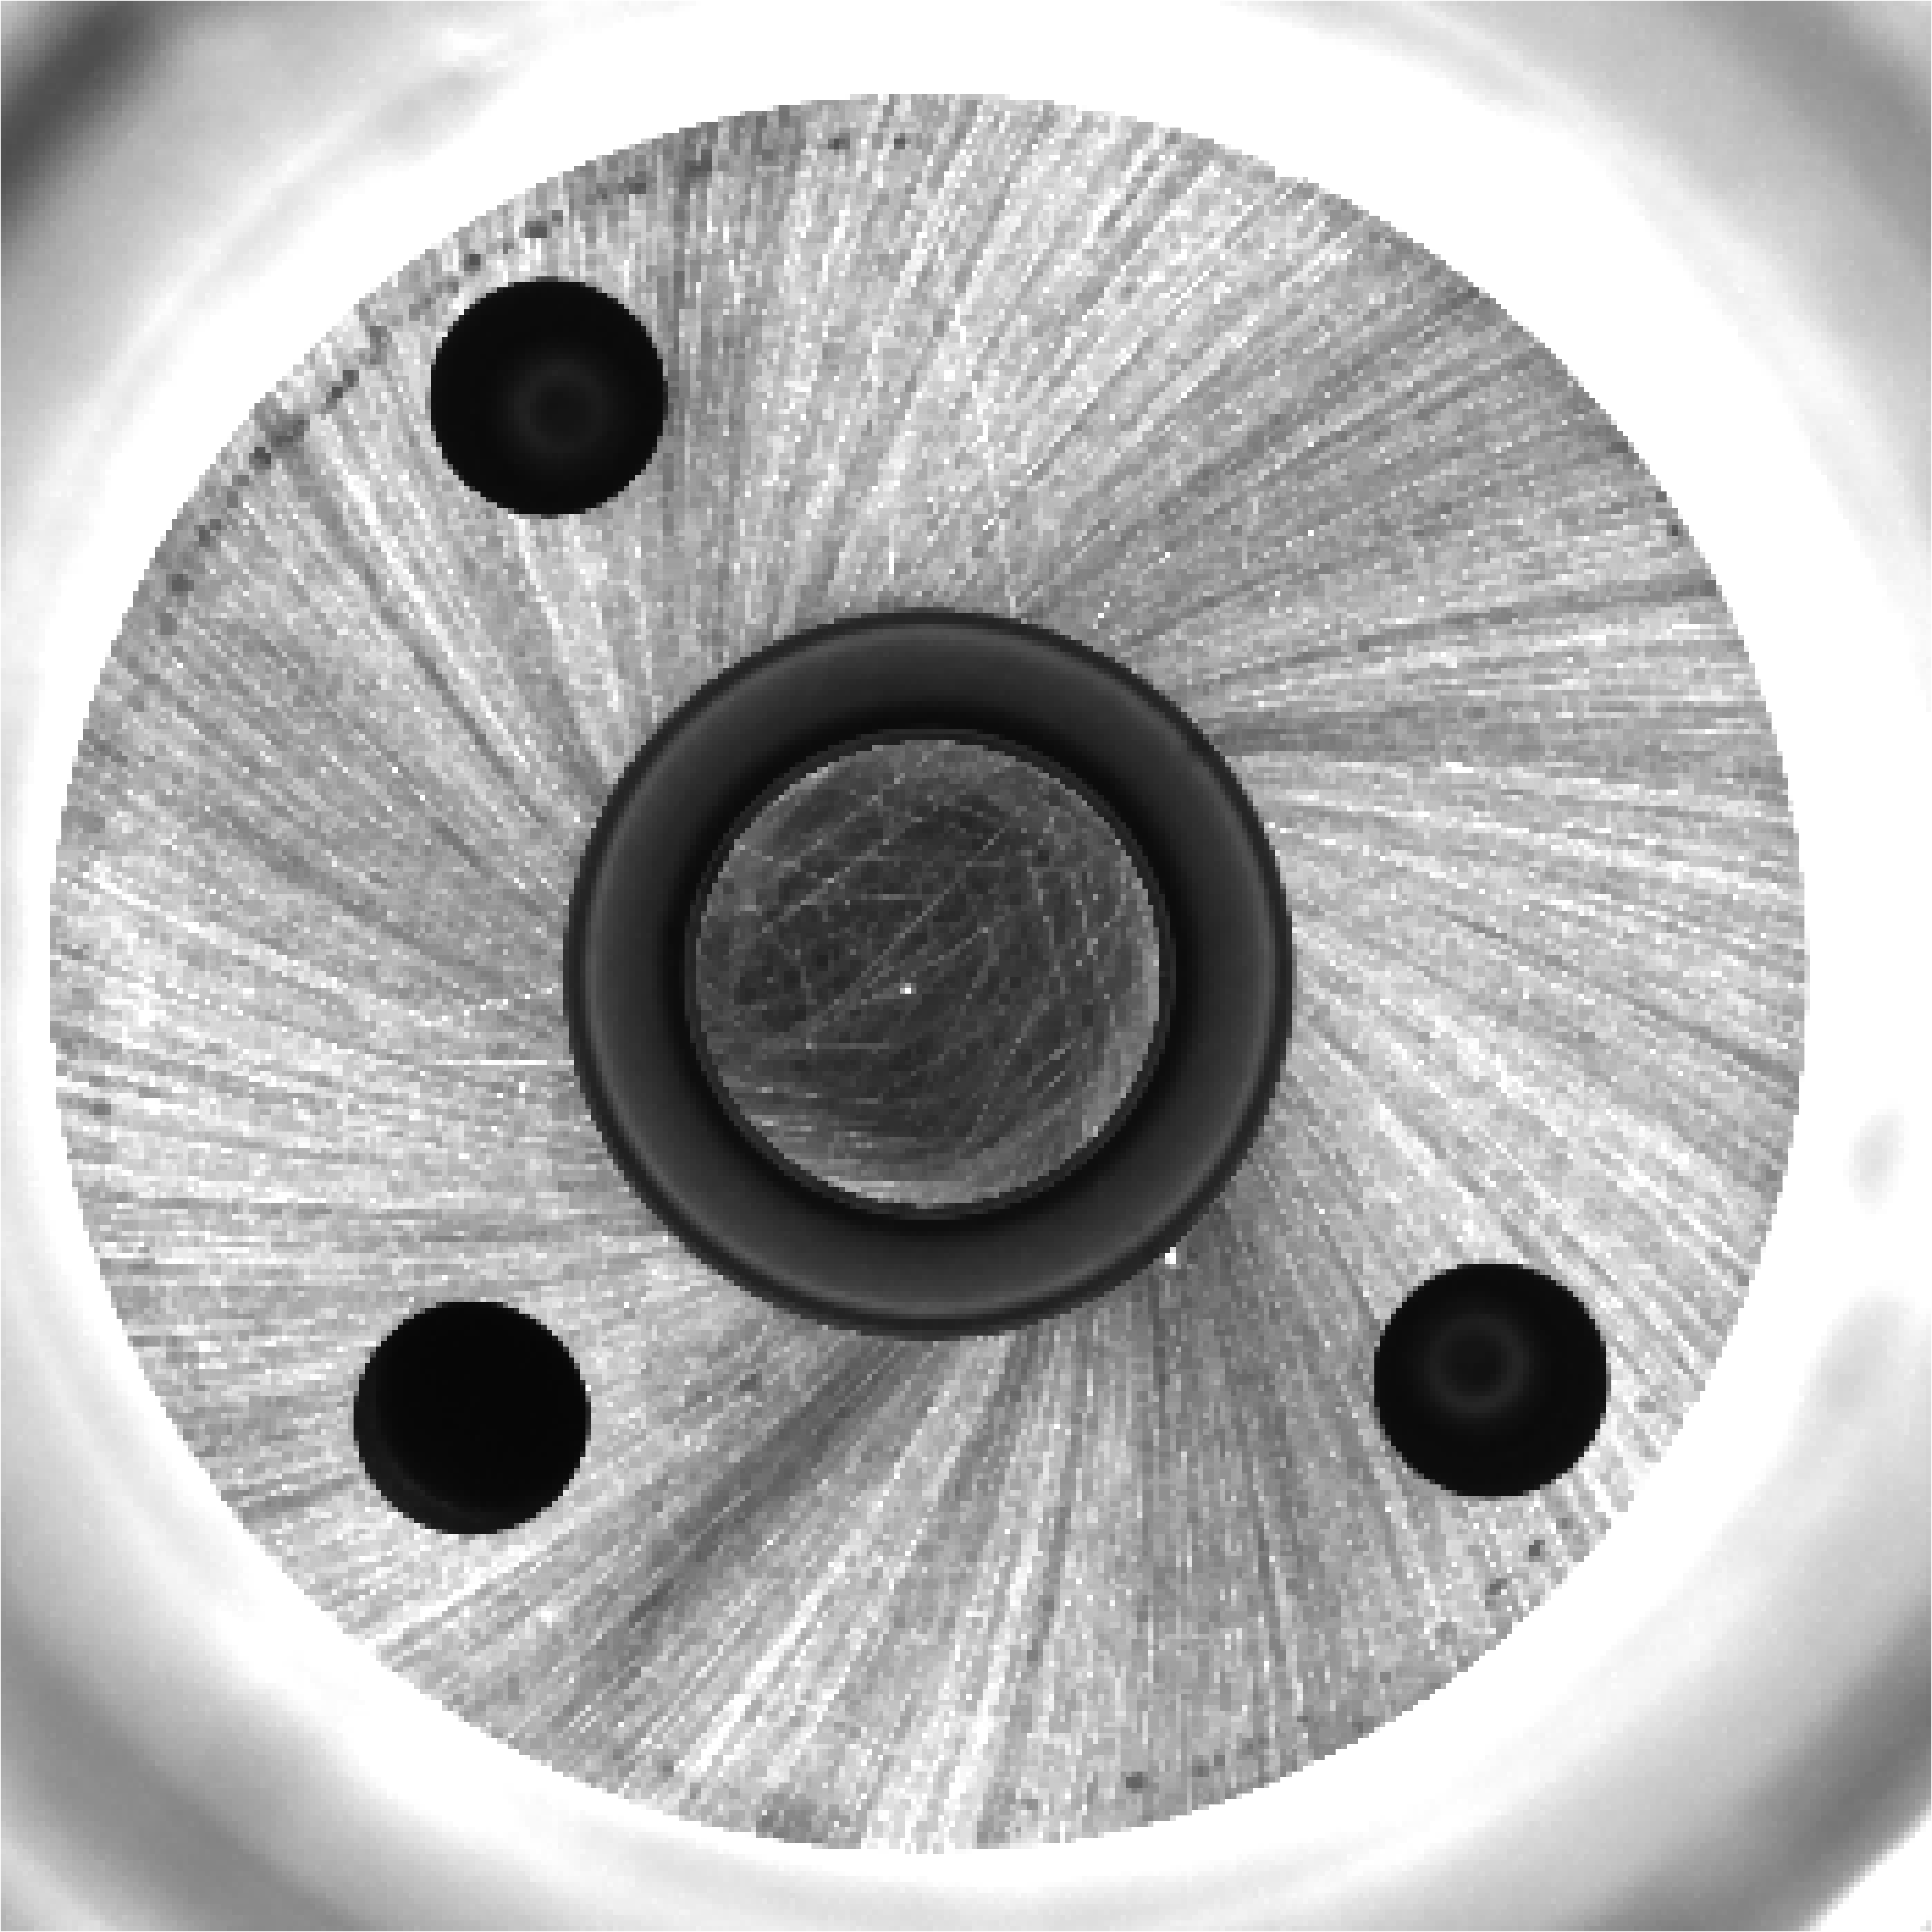
\includegraphics[scale=0.21]{Images/Image0000_closed.png}
	\caption{Imagem após aplicação de filtro de \textit{closing}}
	\label{fig:imClosed}
\end{figure}

\begin{figure}[h]
	\centering
	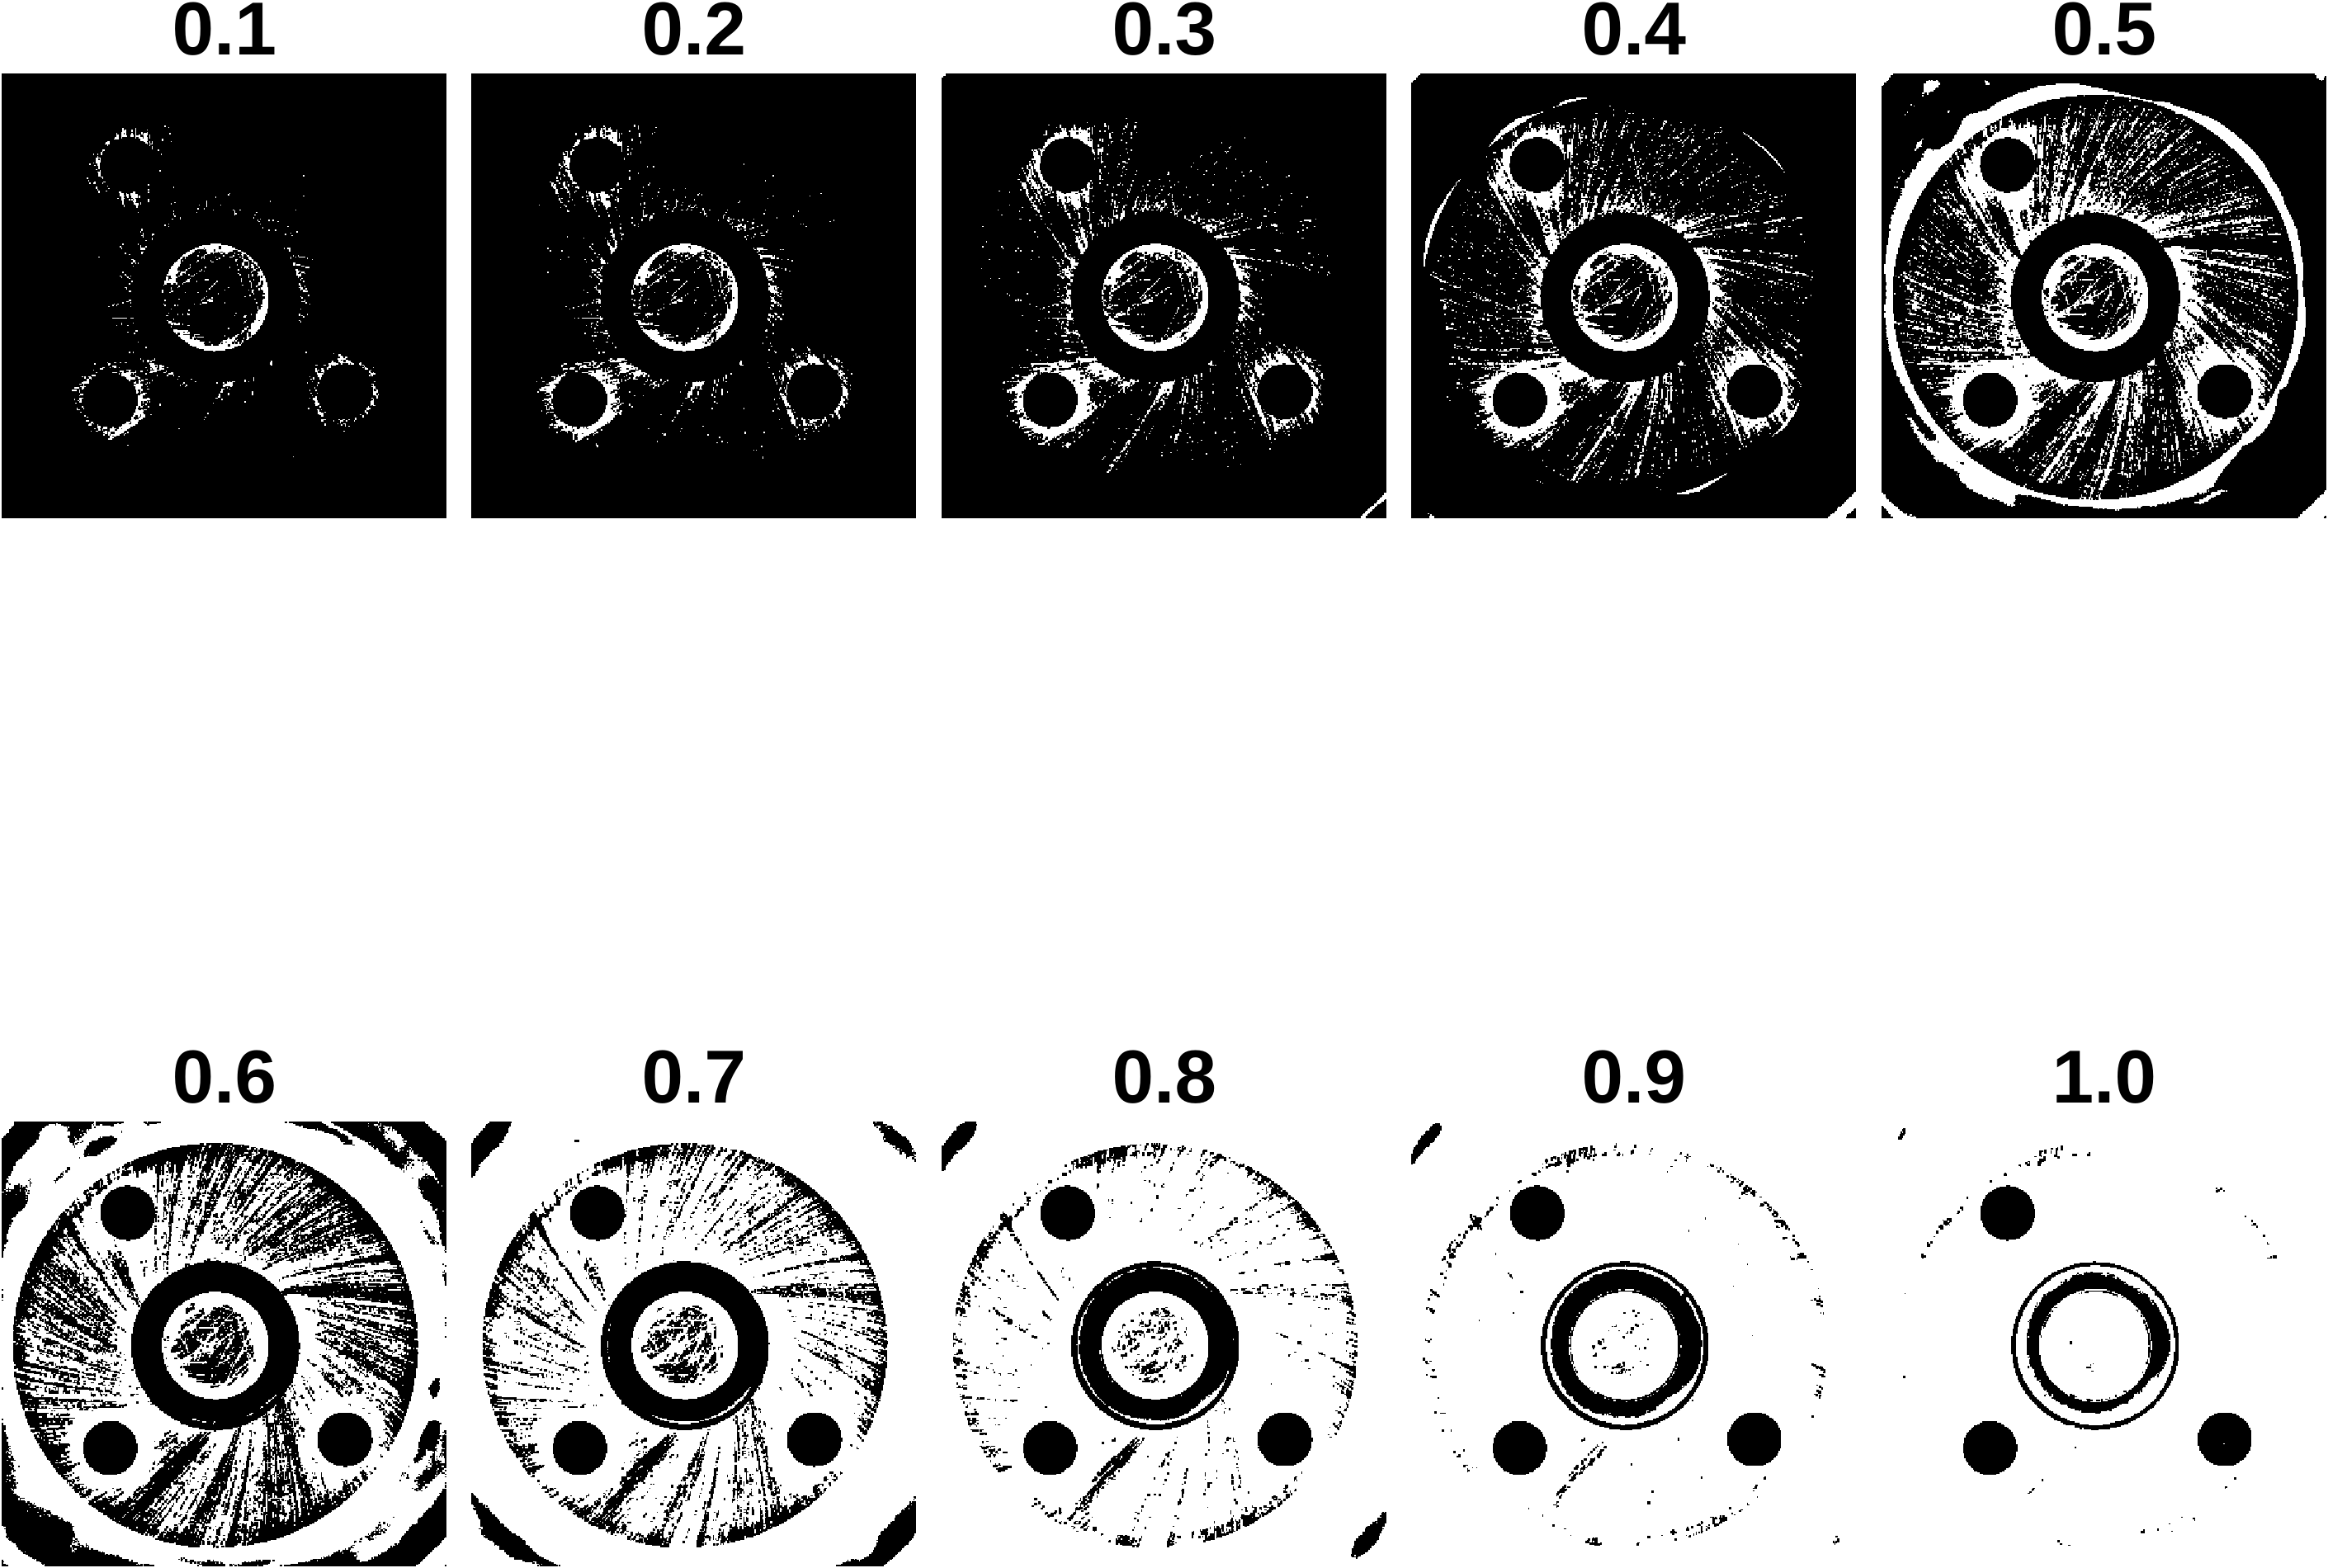
\includegraphics[scale=0.70]{Images/Image0000_sensitivity.png}
	\caption{Imagens binarizadas com diferentes níveis de sensibilidade}
	\label{fig:sensivities}
\end{figure}

\subsubsection{Segmentar os círculos} esta seção apresenta as etapas para segmentação dos círculos na imagem, conforme demonstrado no Código \ref{lst:codigo-segmentation}. Inicialmente, foi definida a variável de sensibilidade como 1,0, de acordo com a análise realizada no Código \ref{lst:codigo-filtering}, e estabelecidas as variáveis de cores para visualização dos círculos (verde) e dos textos na imagem (branco e azul). Em seguida, a imagem foi binarizada utilizando a função \textit{imbinarize} com o método adaptativo. Após a binarização, empregou-se a função \textit{imfindfircles} para detectar os círculos na imagem, especificando o intervalo de raio entre 50 e 200 \textit{pixels} e definindo a polaridade dos objetos como escura. Posteriormente, a função \textit{viscircles} foi utilizada para visualizar os círculos encontrados. Por fim, a Figura \ref{fig:segmented} apresenta a imagem após as etapas de segmentação.

\begin{lstlisting}[caption={Segmentação dos círculos escuros}, label={lst:codigo-segmentation}]
% Select sensitivity to segmentation 
% Select colors to draw circles and text
sensitivity = 1;
edgeColor = [0 1 0];
backgroundColor = [0 0 1];
textColor = [1 1 1];

% Segment image and compute area
imSegmented = imbinarize(imClosed, "adaptive", ...
		      "Sensitivity", sensitivity); 
[c, r] = imfindcircles(imSegmented, [50,200], ...
  	  	 "ObjectPolarity", "dark");

% Show images and circles found
figure; imshow(imNozzle);
title('Original');
figure; imshow(imSegmented);  
viscircles(c, r, "EdgeColor", edgeColor);
title('Segmented');
\end{lstlisting}

\begin{figure}[b]
	\centering
	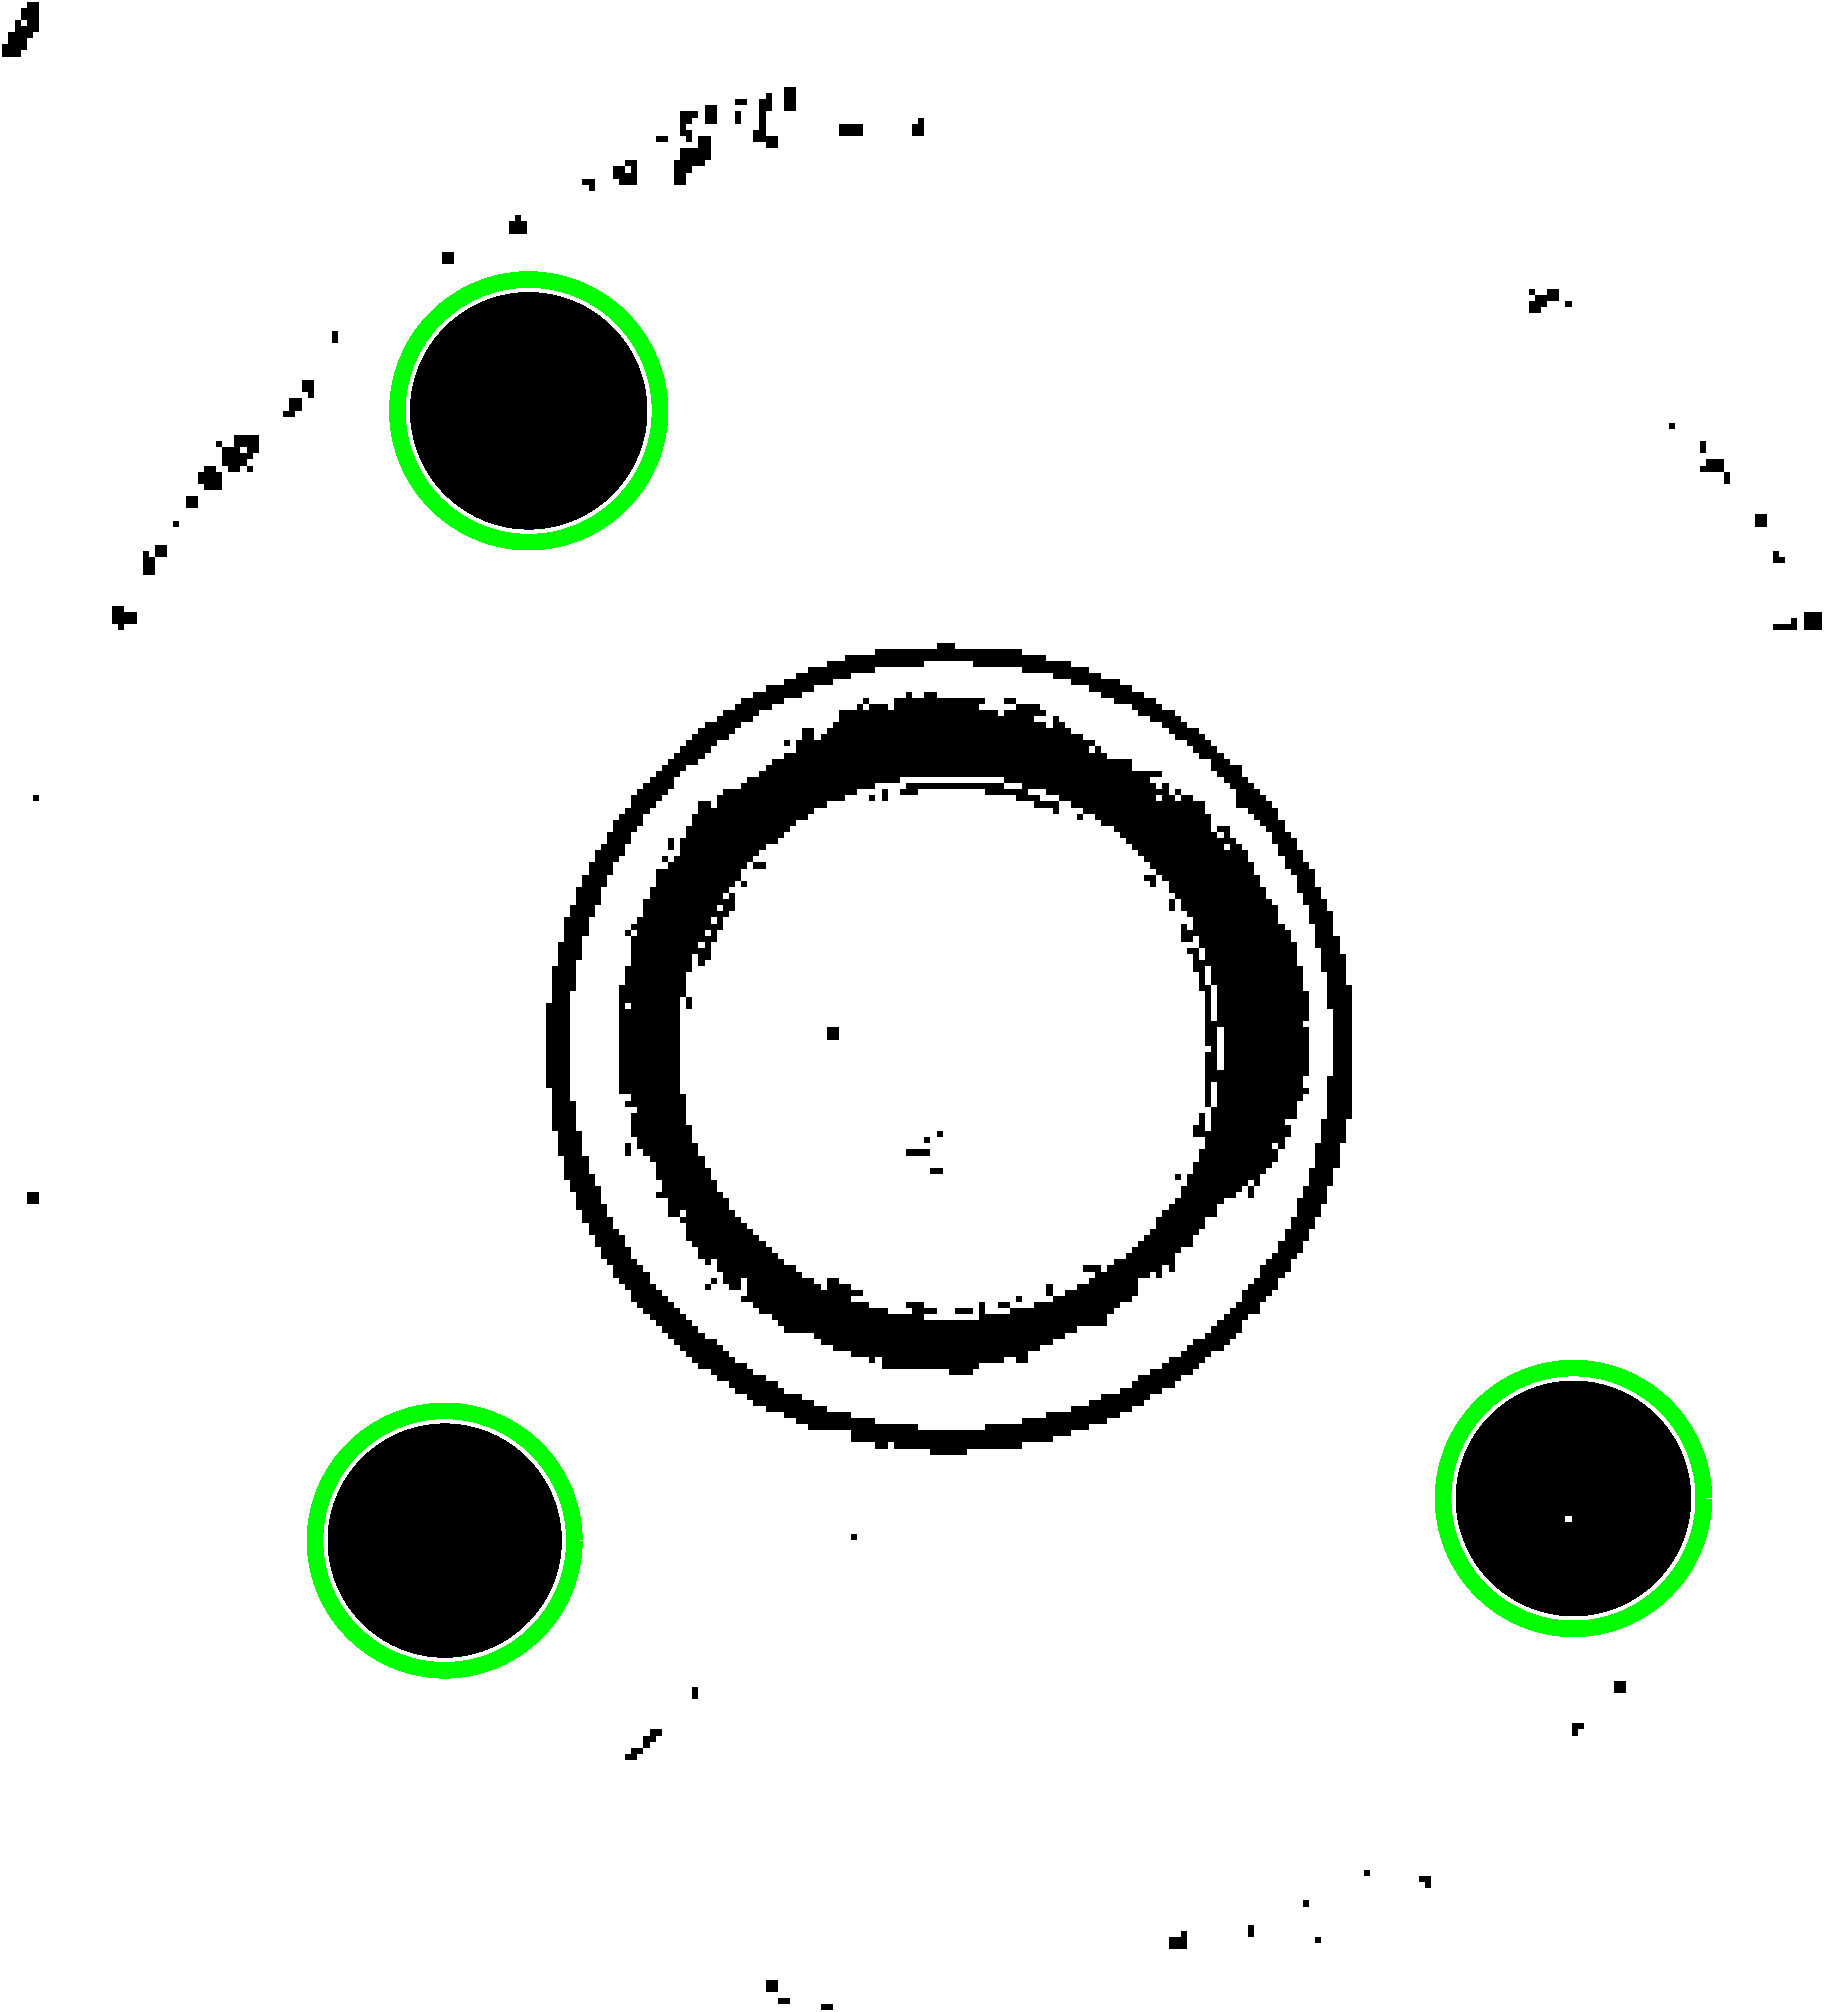
\includegraphics[scale=0.70]{Images/Image0000_segmented.png}
	\caption{Imagem após segmentação e detecção dos círculos escuros}
	\label{fig:segmented}
\end{figure}

\subsubsection{Calcular os ângulos dos círculos} esta seção apresenta as etapas para o cálculo do ângulo de cada círculo encontrado, conforme demonstrado no Código \ref{lst:codigo-compute-angle}. Primeiramente, realizou-se o cálculo dos ângulos dos círculos em relação ao centro da imagem. Como a imagem possui dimensões de 1400x1400 \textit{pixels}, o centro está localizado na coordenada (700, 700). Para realizar o cálculo, utilizou-se a função \textit{atan2}, que retorna o valor de ângulo em radianos, posteriormente convertido para graus com a função \textit{rad2deg}. Por fim, o valor do ângulo obtido é exibido na imagem, seguindo as cores especificadas no Código \ref{lst:codigo-segmentation}, como ilustrado na Figura \ref{fig:compute-angle}.

\begin{lstlisting}[caption={Cálculo dos ângulos em relação ao centro da imagem}, label={lst:codigo-compute-angle}]
% Get number of circles
numOfCircles = size(c, 1);

% Image center
imCenterX = 700;
imCenterY = 700;
	
% Compute and show angles
hold on;
for i=1:1:numOfCircles
	% Draw circle contour
	x = c(i, 1);
	y = c(i, 2);
	
	% Compute angles related to the center 
	theta = atan2(y - imCenterX, x - imCenterY);
	deg = rad2deg(theta);
	text(c(i, 1)+r(i), c(i, 2)+r(i), ...
		 num2str(i)+"="+num2str(deg) + '\circ', ...
		 "BackgroundColor", backgroundColor, ...
		 "Color", textColor, "FontWeight", "bold");
end
hold off;
\end{lstlisting}

\begin{figure}[h]
	\centering
	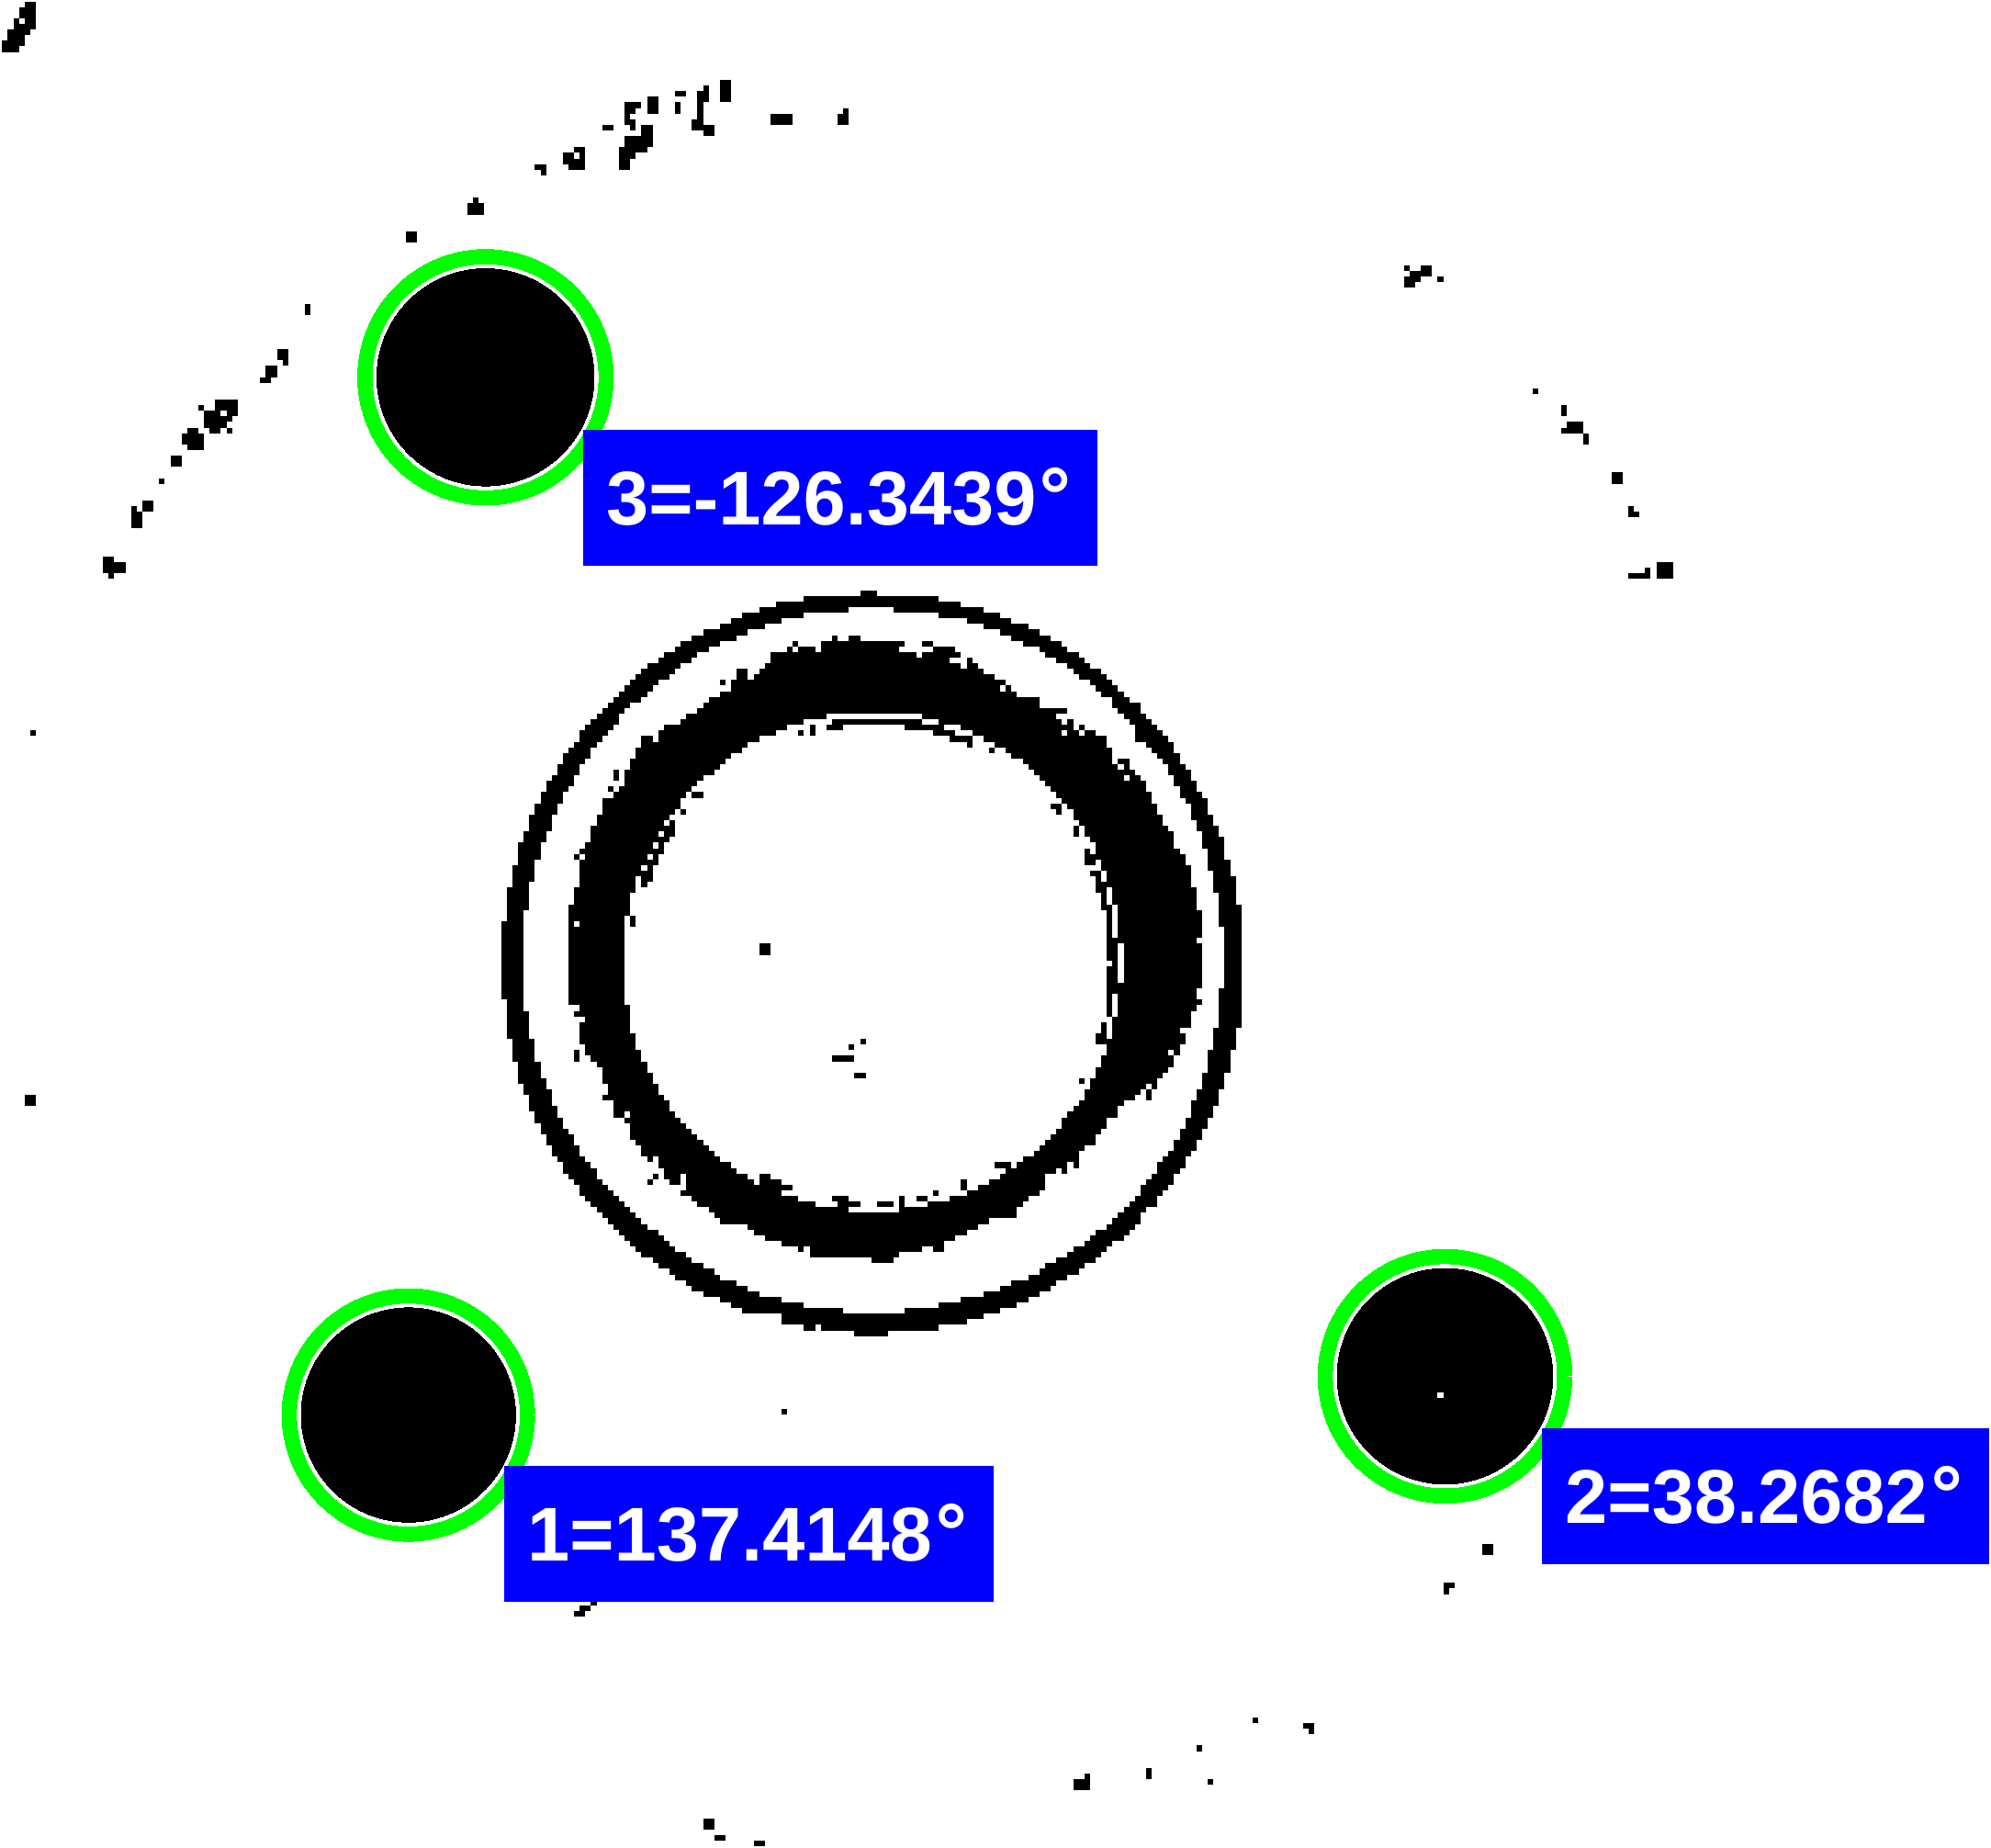
\includegraphics[scale=0.70]{Images/Image0000_computed.png}
	\caption{Imagem após o cálculo dos ângulos}
	\label{fig:compute-angle}
\end{figure}

\section*{Considerações Finais}
Este trabalho teve como objetivo demonstrar a aplicação de técnicas de processamento de imagens para a detecção de furos na superfície de vedação de bicos injetores diesel. Os filtros morfológicos e as funções utilizadas comprovaram o potencial dessas abordagens para aplicações de gravação a laser voltadas à rastreabilidade de produtos.

Após a detecção dos furos e o cálculo de seus ângulos, é possível transferir esses dados para uma gravadora a laser por meio de protocolos de comunicação industrial. Dessa maneira, garante-se que a gravação ocorra na área mais apropriada, que, nesse caso, corresponde à maior região livre de furos ou à maior distancia angular entre dois furos. 

%%%%%%%%%%%%%%%%%%%%%%%%%%%%%%%%%%%%%%%%%%%%%%%%%%%%%%%%%%%%%%%%%%%%%%%%%%%%%%%%%%%%%%%%%%%%%%
%\section*{References}
\bibliographystyle{IEEEtran}
\bibliography{references}

%\begin{thebibliography}{00}
%\end{thebibliography}

%\vspace{125pt}
%\color{red}
%IEEE conference templates contain guidance text for composing and formatting conference papers. Please ensure that all template text is removed from your conference paper prior to submission to the conference. Failure to remove the template text from your paper may result in your paper not being published.

\end{document}
